%% paper.tex
%% V1.4b
%% 2017/03/05
%% by HSNL, NTHU

\documentclass[conference]{IEEEtran}

\usepackage{graphicx}
\usepackage{indentfirst}
\usepackage{cite}
\usepackage{url}
\usepackage{hyperref}
\usepackage{enumerate}
\usepackage[flushleft]{threeparttable}
\usepackage[super]{nth}
\usepackage[none]{hyphenat}
\usepackage[OT1]{fontenc}


\begin{document}

\title{A Novel vCPE Framework for Enabling Virtual Network Functions with Multiple Flow Tables Architecture in SDN switches}

\author{
\IEEEauthorblockN{
Nen-Fu Huang\IEEEauthorrefmark{1},
Chi-Hsuan~Li\IEEEauthorrefmark{1},
Chia-Chi~Chen\IEEEauthorrefmark{1},
I-Hsien~Hsu\IEEEauthorrefmark{1},
Che-Chuan~Li\IEEEauthorrefmark{1}, and
Ching-Hsuan~Chen\IEEEauthorrefmark{2}
}

\IEEEauthorblockA{
\IEEEauthorrefmark{1}
Department of Computer Science National Tsing Hua University, Hsinchu, Taiwan
}
\IEEEauthorblockA{\IEEEauthorrefmark{2}
Institute of Communication Engineering National Tsing Hua University, Hsinchu, Taiwan
}
}

% make the title area
\maketitle

\begin{abstract}
The virtual Customer Premise Equipment (vCPE) concept has been proposed recently to reduce OPEX and CAPEX. Software-defined networking (SDN) and network functions virtualization (NFV) are key roles for this innovation. This paper proposes a vCPE framework enables deploying VNFs as edge of network. These VNFs are achieved by the synergies between a VNF controller on the cloud and an SDN switch at the edge. A multiple flow table management model is also proposed to implement virtual network functions. Through the proposed vCPE framework, the customer only needs a generic SDN switch at local network and very easy to subscribing different network services, such as Firewall, NAT, DHCP, and applications quality of service (QoS) by a browser-based dashboard. Experiments are conducted to evaluate the performance of VNFs implemented by the proposed multiple flow table management model. The flexibility of framework to integrate with other application classification systems, such as IDS or IPS, is also demonstrated.

\end{abstract}

% Note that keywords are not normally used for peerreview papers.
\begin{IEEEkeywords}
Multiple flow tables, NFV, SDN, vCPE
\end{IEEEkeywords}

\IEEEpeerreviewmaketitle{}





\section{Introduction}
In recent times, researchers have shown an increasing interest in evolving network infrastructures.
Software-defined networking (SDN) and network functions virtualization (NFV) are key roles for this evolution.
SDN \cite{sdn-mckeown-2009-talk, sdn-newnorm, sdn-road, sdn-compre-survey} has been widely studied for almost a decade since the first OpenFlow \cite{openflow-mckeown-2008, openflow-spec} article had be presented in 2008.
The main concept of SDN is separating data plane and control plane to enable smart control on switch and give a brand-new viewpoint on network research, and makes innovation on industries.

As SDN was developed, NFV \cite{nfv-wp, etsi-nfv-archi, nfv-survey} has been introduced by Telco operators at the same time.
The network services offered by operators were previously performed by specific hardware appliances and it is difficult to decrease the OPEX and CAPEX on service deployment and management.
In this context, NFV is proposed to innovate in the service delivery arena.
The concept of NFV is to reduce the coupling between network functions (NFs) and hardware devices.
Virtual Customer Premise Equipment (vCPE) \cite{nec-vcpe, vcpe-enhance} is one of the network services which benefited from NFV \cite{etsi-nfv-usecase}.

In the progress of vCPE development, SDN is not involved at first.
Most of previous researches focused on other technology to virtualize and deploy the CPE node \cite{virtual-rg, security-vgw, design-vrgw, nfv-hgw-surrogate, linux-cpe, nfv-resoure-contrain-cpe}.
Cloud4NFV \cite{cloud4nfv, cloud4nfv-telco}, proposed by Portugal Telecom, started to use SDN technology on designing virtual CPE management and organization (MANO) platform.
Italy Telecom also proposed NetFATE \cite{netfate}, which is a network function deploy-to-edge model in which the NFs are designed by SDN and perform by SDN switch. However, NetFATE merely tested the scenario of virtual firewall which lacked sufficient experimental results for other scenarios under NetFATE platform.

Inspired from these two frameworks, a vCPE framework with six major virtual network functions are proposed in this paper, attempting to replace hardware-based CPE.
Nevertheless, when the NFV is deployed at network edge (SDN switch), it is very difficult and not efficient to implement multiple virtual network functions in a single OpenFlow Table \cite{multiple-flow-table}. In this paper, a multiple OpenFlow table mechanism is also proposed to implement multiple network functions. The performance of new VNF implemented by the proposed mechanism is evaluated by comparing with the single-table mechanism. Based on the proposed vCPE framework, this new VNF can also be deployed to the network edge easily.






\section{vCPE System}
\subsection{Overview of Network Functions} \label{ssec:desc_nfv_overview}
Our network functions are designed with SDN-enabled NFV architecture concept \cite{sdn-enabled}, using the synergies between computing infrastructures (NFVs) and network infrastructures (NFVIs) \cite{etsi-nfv-terminology, etsi-nfv-infra}.
An NFV is mainly used for addressing stateful processing and NFVI is used for stateless processing. In our architecture, we use an SDN controller as NFV and an SDN switch as NFVI.
By using the advantages of this architecture, we can assign stateless or light-weight state work to the SDN switch (e.g., packet filtering and packet counting) to reduce the load on the computing resources. If we want to update our service, we are required to update only the stateful component, because the stateless component merely follows the commands from the stateful component.




\subsection{Service Deployment Model}
Unlike related studies that explored the virtualization of network function in PE devices \cite{vcpe-enhance} or used service-chains in data center to achieve vCPE services \cite{ericcson-vcpe}, we introduced a network function service deployment model based on the NetFATE (Network Function at the Edge) approach \cite{netfate}; the architecture of the model is presented in Fig. \ref{fig:desc_service_deployment}. Because computing infrastructures involves algorithms and policies and the generic network devices perform only stateless processing, the customers need to simply purchase a general SDN switch for their home gateway. They can obtain a different network function service by subscribing to a different VNF controller through our vCPE platform.

Fig. \ref{fig:desc_service_deployment} illustrates the service deployment model. Each green area is a local network domain of the customer. An SDN switch is presented at the gateway of this domain. The customer can subscribe to our vCPE service through our dashboard. After subscription, the vCPE system creates a new Docker container that an SDN controller is run. The customer only needs to set up the gateway SDN switch to connect the SDN controller through the OpenFlow protocol; thereafter, the switch executes the service.

\begin{figure}[!t]
\centering
\includegraphics[width=0.4\textwidth]{./figures/desc_service_deployment}
\caption{Service deployment model.}
\label{fig:desc_service_deployment}
\end{figure}



\subsection{vCPE System Architecture}
The architecture (Fig. \ref{fig:desc_vcpe_framework}) is adapted from the NFV-MANO architectural framework in \cite{etsi-nfv-mano}, including an infrastructure controller, an infrastructure orchestrator, a cloud database, VNF controllers and a VNF Orchestrator. Each component is introduced in the following subsection.

\begin{figure}[!t]
\centering
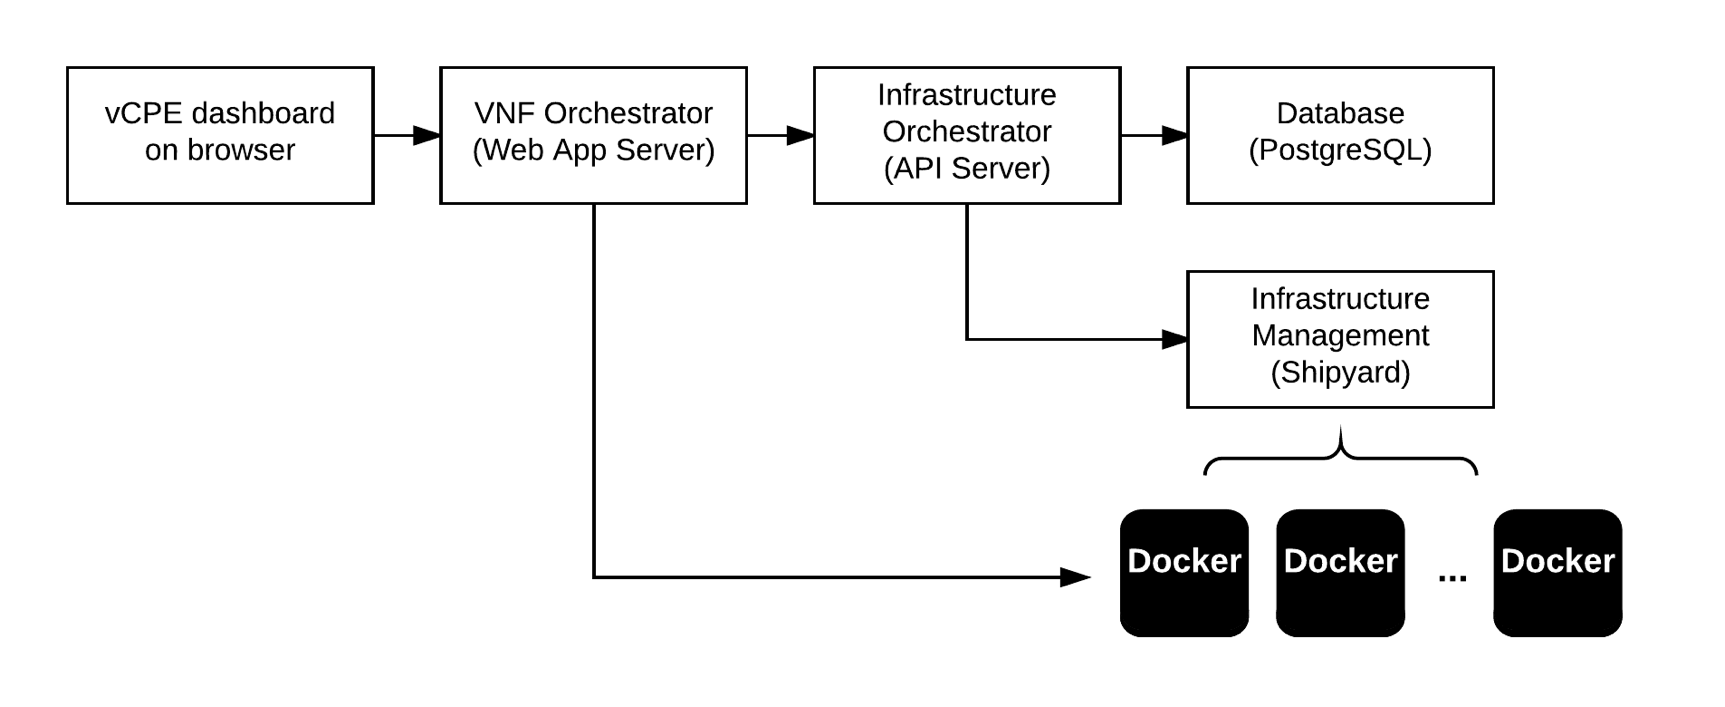
\includegraphics[width=0.4\textwidth]{./figures/desc_vcpe_framework}
\caption{Architecture of the vCPE system.}
\label{fig:desc_vcpe_framework}
\end{figure}

\subsubsection{Infrastructure Controller}

The infrastructure controller comprises a Docker management server and follows the request from the infrastructure orchestrator to create, delete, start, stop, and inspect containers.

\subsubsection{Infrastructure Orchestrator}

The infrastructure orchestrator automates the workflows of service deployment. When a customer subscribes to our service, the infrastructure orchestrator first authenticates the customer, calls the infrastructure controller to create a container for the customer, and then updates the information in the cloud database.

\subsubsection{Cloud Database}
The cloud database is used for restoring the meta data of our vCPE services, which include each customer’s credentials, customer's container/VM settings, and virtual CPE service states.

\subsubsection{VNF Controllers}
VNF controllers comprises an SDN controller developed using Ryu framework \cite{ryu} and a remote launcher module. Once the infrastructure controller creates the container, the remote module will initially run, waiting for requests from VNF Orchestrator. The details of an SDN controller design are presented at Section \ref{sec:mft}.

\subsubsection{VNF Orchestrator}
The VNF orchestrator provides web-based UI for vCPE services management and configuration. Through the VNF orchestrator, customers can subscribe to the desired service. After receiving the subscription message, the VNF orchestrator requests the infrastructure orchestrator to create a new VNF controller, and then sends the virtual CPE configuration to the new VNF controller. Based on configuration demands under different conditions, the network administrator can select any of the listed network functions on the dashboard, such as Firewall, NAT, DHCP, and quality of service (QoS) management.





\section{Network Function With Multiple Flow Table Management Model} \label{sec:mft}

\begin{figure*}[!t]
\centering
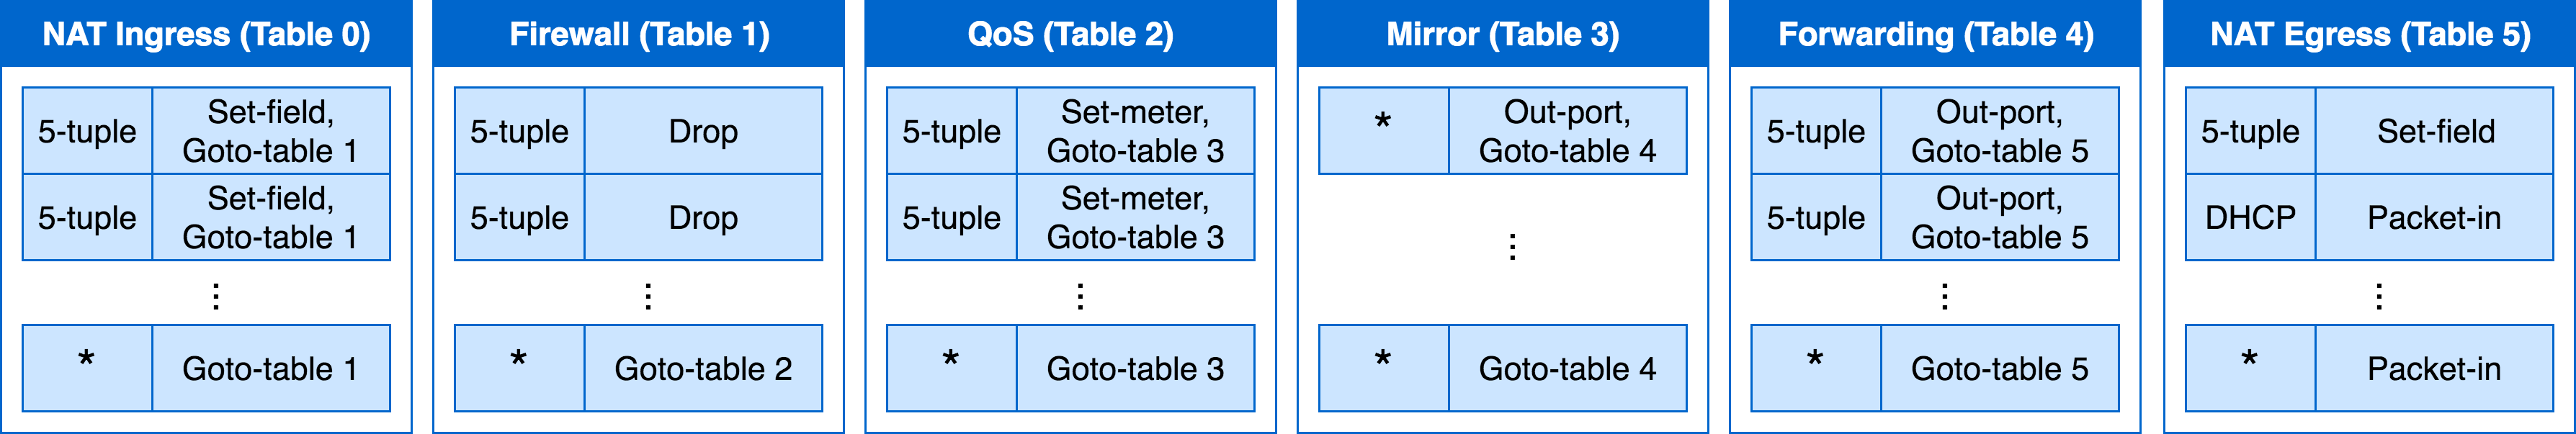
\includegraphics[width=\textwidth]{./figures/mft_table_overview_v4.png}
\caption{Flow table order of vCPE service.}
\label{fig:mft_table_overview}
\end{figure*}



\subsection{Multiple Flow Tables Strategy}
In subsection \ref{ssec:desc_nfv_overview}, we have introduced the SDN-enabled NFV design architecture. The network functions are managed through cooperation between the SDN controller on the cloud and SDN switch at the local network gateway. The controller transforms the network functions into a series of OpenFlow rule requests and sends it to the SDN switch. Following the orders from the controller, the SDN switch inserts the rules into its flow tables, examines the incoming packets against the flow entry match fields, and executes the actions in matching rules. The flow table \cite{sdn-ft} defines all matching and corresponding processing, thus playing an important role in the executive network function.

We found that a single flow table restricts the implementation of our network functions. In \cite{multiple-flow-table}, two conditions under which a single flow table is too restrictive were reported. The first is a condition where a single packet must perform independent actions based on matching with different fields. The second is a condition where the packet requires two-stage processing. So, if we want to implement two network functions, like QoS and firewall, the rules of SDN switch are very complex. To resolve both restrictions, we implemented the network functions by using a multiple flow table strategy.

Before discussing the multiple flow table strategy, we introduce the pipeline of OpenFlow flow table first \cite{openflow-spec}. The processing of each packet always starts at the first flow table. When being processed by a flow table, the packet is matched the flow entries of the flow table and adds corresponding action to the instruction set. The packet can execute the instruction set immediately, or execute after finishing the journey in switch. A flow entry can direct a packet to next table by go-to action. In our multiple flow table management model, we set the ``go to next table'' action as the table-miss action. Therefore, the packet is processed table-by-table in a certain sequence.

In a multiple flow table strategy, it is most important to determine which rules of the flow table should be inserted into. We used the type of network function as a demarcation, that is, SDN applications responsible for specific network functions inserted rules into one specific flow table to enable us to focus on the design of the network function itself. However, the order of the flow table and the sequence of the network functions become crucial. This can be addressed by considering the type of match and action in the rules generated by the network function.

The network functions of vCPE services are the firewall, NAT, DHCP, forwarding, traffic mirroring and QoS. The order of each function was determined as shown in Fig. \ref{fig:mft_table_overview} (note that the flow tables are counted from zero). In the following sections, we introduce the method of implementing these network functions, the type of rules to be inserted into the SDN switch, and the effect of these rules on deciding the order of the flow tables.



\subsection{Service Control}
Service control is used to enable or disable services. To enable a service, the table-miss rule should be modified. A packet-in rule is always placed in the flow table of the last active service as a table miss in case there is no corresponding rule. To enable the service chain, the rules of each service except the last service contain an additional action, ``go to next table'', which enables the packets to continue to pass through all active services.

To disable a service, we merely add an enforce rule. Each enforce rule has the highest priority with the action, ``go to next table''. It indicates that packets still pass through the disabled service’s table, but ignore other rules and proceed to the next flow table.



\subsection{Firewall}
The firewall service can dynamically block traffic based on MAC address, IP and layer4 ports.
In our multiple flow table model, the firewall service is located in flow table 1 because once packets are detected by the blocking rules, they do not need to be applied to any other services.
The action of the firewall is different from those of other services, because in other services, irrespective of the actions taken with the packets, the packets must proceed to the next flow table.



\subsection{NAT}
The NAT service allows numerous hosts to use one public IP address for connecting to the network.
Following is an example that illustrates the workflow of our NAT service.
For an outgoing packet of a new connection, the SDN switch does not have any flow entry in the flow table, and hence, a packet-in event is triggered initially.
In controller, the source IP and source port number of the outgoing packet are modified to a public IP address and a new port number is remapped for NAT service by Set-Field action.
For the incoming packet, the destination IP address and destination port number are modified to fit the private IP address and port number.
Subsequently, the SDN controller adds these flow entries to the SDN switch.

In the single flow table framework, two rules must be added to the SDN switch to match the outgoing and incoming situations.
First, we predicted that the NAT service must be placed in the last table of the multiple flow table framework because the NAT service must set the packet header fields and enable connection to the outside network.
Most importantly, the SDN switch is placed according to the order of tables to match the field.
The outgoing and incoming situations must be considered.
In consideration of all the aforementioned factors, we place the NAT service in the first and last tables in our multiple flow table framework.



\subsection{DHCP}
The DHCP service implements the DHCP protocol to dynamically assign IP addresses to hosts.
Since the DHCP merely needs one Packet-in rule to forward DHCP packets to controller, a specific flow table for the DHCP service is not required.
When the service is disabled, the DHCP rule is deleted, and the packets continue to pass through our service chain.
The subsequent DHCP packets can reach other DHCP servers by forwarding service.



\subsection{Traffic Mirroring} \label{ssec:mirror}
The traffic mirroring service could make the manager to specify the output port to mirror the packet flow.
It could make the network manager monitor the network situation easily.
In our multiple flow table architecture, we use this service to mirror the packet flow to classifier which could identify the application.
The QoS service could use the classified result to limit the application.



\subsection{Forwarding} \label{ssec:forwarding}
In the forwarding service, when the first packet in a new connection is incoming, a packet-in event occurs because no corresponding rule is present.
When the controller receives the packet, it records the IP-layer information, including the source IP address, destination IP address, input port number, source MAC address, and destination MAC address.
By using the recorded information, the controller can install a 5-tuple forwarding rule with the out-port action for this connection, and the subsequent packets do not need to undergo the packet-in event.
The 5-tuple comprises the source IP address, destination IP address, network layer protocol, source layer 4 port, and destination layer 4 port.



\subsection{QoS}
Quality of Service (QoS) provides two strategies: hosts rate limitation and applications rate limitation.

\subsubsection{Hosts Rate Limitation}
To implement the rate limiting for hosts, we use meter, which is defined within OpenFlow protocol 1.3, to set the limitation in the specific bandwidth. Therefore, we will create a meter for a desired bandwidth and assign the flows of target host with it.


\subsubsection{Rate Limitation of Applications}

In this strategy, we integrated a flow classification engine \cite{che-chuan-apnoms} to identify the flow belongs to which application.
To avoid some applications taking up a lot of bandwidth, we can limit the bandwidth for a certain application.
We will mirror the packet to flow classification engine and identify which application belongs to.
If we want to limit a specific application, we just add a 5-tuple rule and same meter to those packets which belong to this application.
As a result, those applications will share the bandwidth by this meter.

\subsubsection{The Order of Forwarding Table and QoS Table}
Because the order of NAT, DHCP, mirroring and the firewall have been determined, we only need to decide the arrangement of QoS and forwarding. Assume that we place the QoS flow table after the forwarding flow table. In addition, we have only two services enabled, forwarding and QoS; therefore, the packet-in rule is in the last flow table of active service, QoS service. Then, suppose that a host is not limited by QoS policies. The first packet is not affected in both arrangements. For the subsequent packets, a difference can be observed. The packets that satisfy the rules in the forwarding flow table can not match the rate limit rules in QoS flow table, because the host is not limited by QoS service; instead. As a result, the packets cause packet-in events by matching the packet-in rule in QoS service. This is unexpected because the packets already get the out-port action from the forwarding service. That is, it is not necessary to send these packets go to controller, and any packet-in event increases the controller’s load.

To reduce this load on the controller, we place the QoS flow table ahead of the forwarding flow table. In this scenario, all packets that pass through the QoS flow table continue to proceed to the forwarding flow table without satisfying any QoS rules. Then, all packets except the first packet are merely forwarded by the forwarding service instead of causing packet-in events. Thus, the controller’s load decreases.




\section{Performance Evaluation}
\subsection{Multiple Table Performance}

\begin{figure}[!t]
\centering
\includegraphics[width=0.4\textwidth]{./figures/evaluation_nat_scenario}
\caption{Multiple Table Performance Evaluation Scenario}
\label{fig:evaluation_nat_scenario}
\end{figure}

\begin{figure}[!t]
\centering
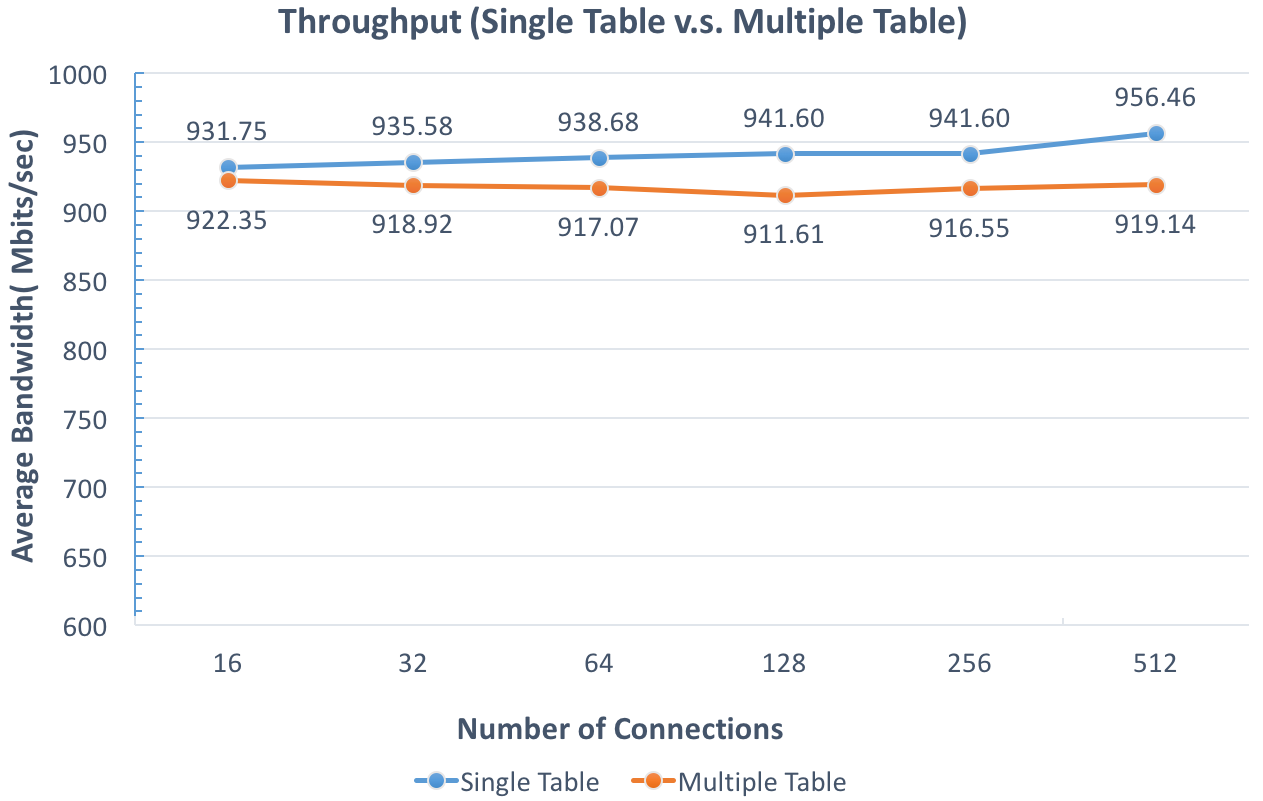
\includegraphics[width=0.4\textwidth]{./figures/evaluation_nat}
\caption{Results of Multiple Table Performance Evaluation}
\label{fig:evaluation_nat_result}
\end{figure}

Implementing a single flow table framework is easier than implementing a multiple flow table framework; however, multiple flow table frameworks are more flexible. To verify the efficiency of the multiple flow table vCPE framework, we conducted an experiment by using the NAT and forwarding service to compare the throughput between single flow table vCPE and multiple flow table vCPE.

An overview of the experimental environment is presented in Fig. \ref{fig:evaluation_nat_scenario}. The NFV controller was run on the Dell PowerEdge R630 rack server, and the EdgeCore AS5712-54X \cite{edge-core-switch} was used as the SDN switch.
We used iPerf \cite{iperf} to generate network traffic. The iPerf server connected the public IP address with 140.114.71.176, and then the iPerf client connected to the SDN switch and was controlled by the NFV controller.
The NFV controller ran the NAT service, but used different frameworks, a single flow table and multiple flow table.

We used iPerf to generate TCP packets and send them to the server from the client.
In this experiment, different number of connections were used to evaluate the performance of the flow tables.
As shown in Fig. \ref{fig:evaluation_nat_result}, the throughput values indicated that the performance for the low number of connections are similar.
But if we increased the number of connections, the difference of performance between the performance of two applications become bigger and bigger.

For each connection, the multiple table application added 4 rules and single table application added merely 2 rules. Since the multiple table applications needed more rules than the other, the throughput of the multiple table framework is worse than the throughput of the single table framework for the large number of connections conditions.
Although the value of multiple table framework is lower than single table framework at the more number of connections, the multiple table framework is more flexible than the single table framework.



\subsection{Evaluation of QoS When Host Bandwidth Is Limited}

Because downloading is a situation that always consumes network resources in practice,
we verify our function by downloading an image of Ubuntu 14.04 that was approximately 1 GB in size.

The NFV controller ran on the Dell PowerEdge R630 rack server and executed QoS.
The Edge-Core AS5712-54X \cite{edge-core-switch} switch was used as the OpenFlow-enabled switch with the PicOS TM r2.6 operating system.
We used a desktop computer as the experimental host to record the bandwidth every 2 seconds.

As shown in Fig. \ref{fig:qos_limit_host}, we started downloading the file without rate limiting and the rate was between 40,000 and 70,000 Kbps.
At the \nth{8} second, we limited the host 1 to 2048 Kbps and host 2 to 1024 Kbps by adding the rule of their MAC address.
Then the bandwidth from host 1 and host 2 is decreasing. Host 1 and host 2 were limited to approximately 2048 Kbps and 1024 Kbps, respectively.
At the \nth{42} second, we change the bandwidth to host 2. That is, we set the bandwidth to host 2 from 1024 Kbps to 5120 Kbps.
We observed that the bandwidth of the host 2 rapidly increased to 5120 Kbps.

\begin{figure}[!t]
\centering
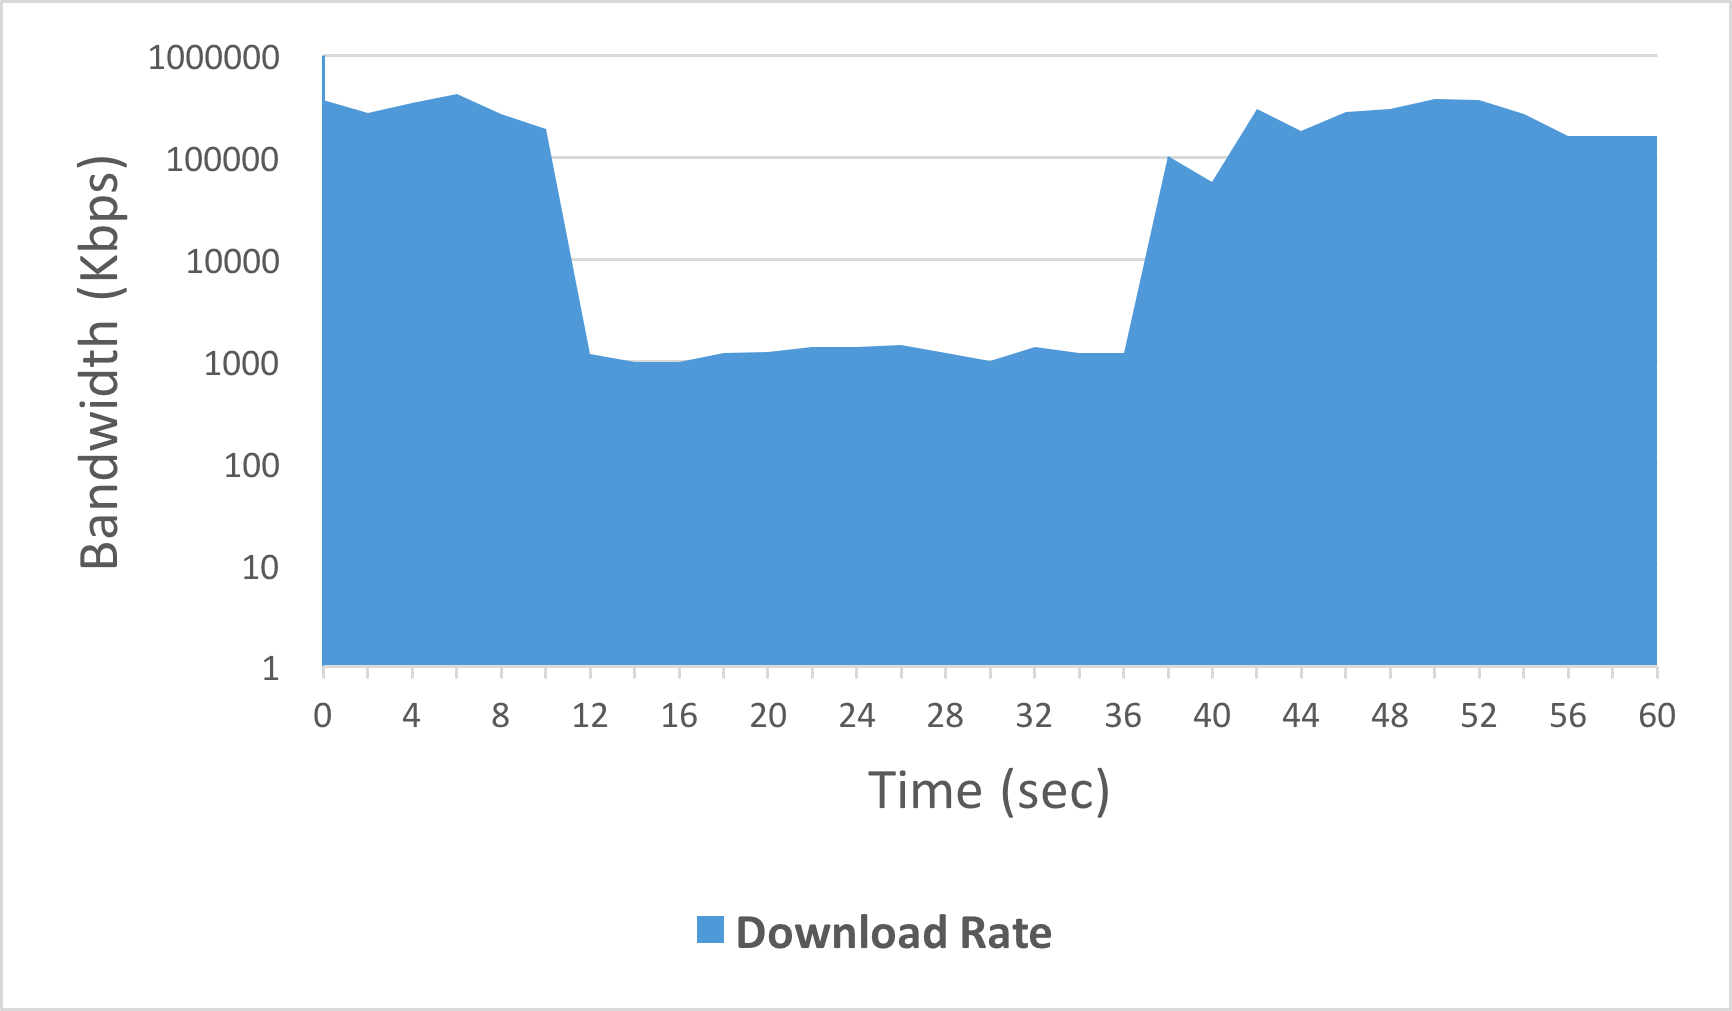
\includegraphics[width=0.4\textwidth]{./figures/qos_limit_host}
\caption{Limiting the download rate of a host.}
\label{fig:qos_limit_host}
\end{figure}

\begin{figure}[!t]
\centering
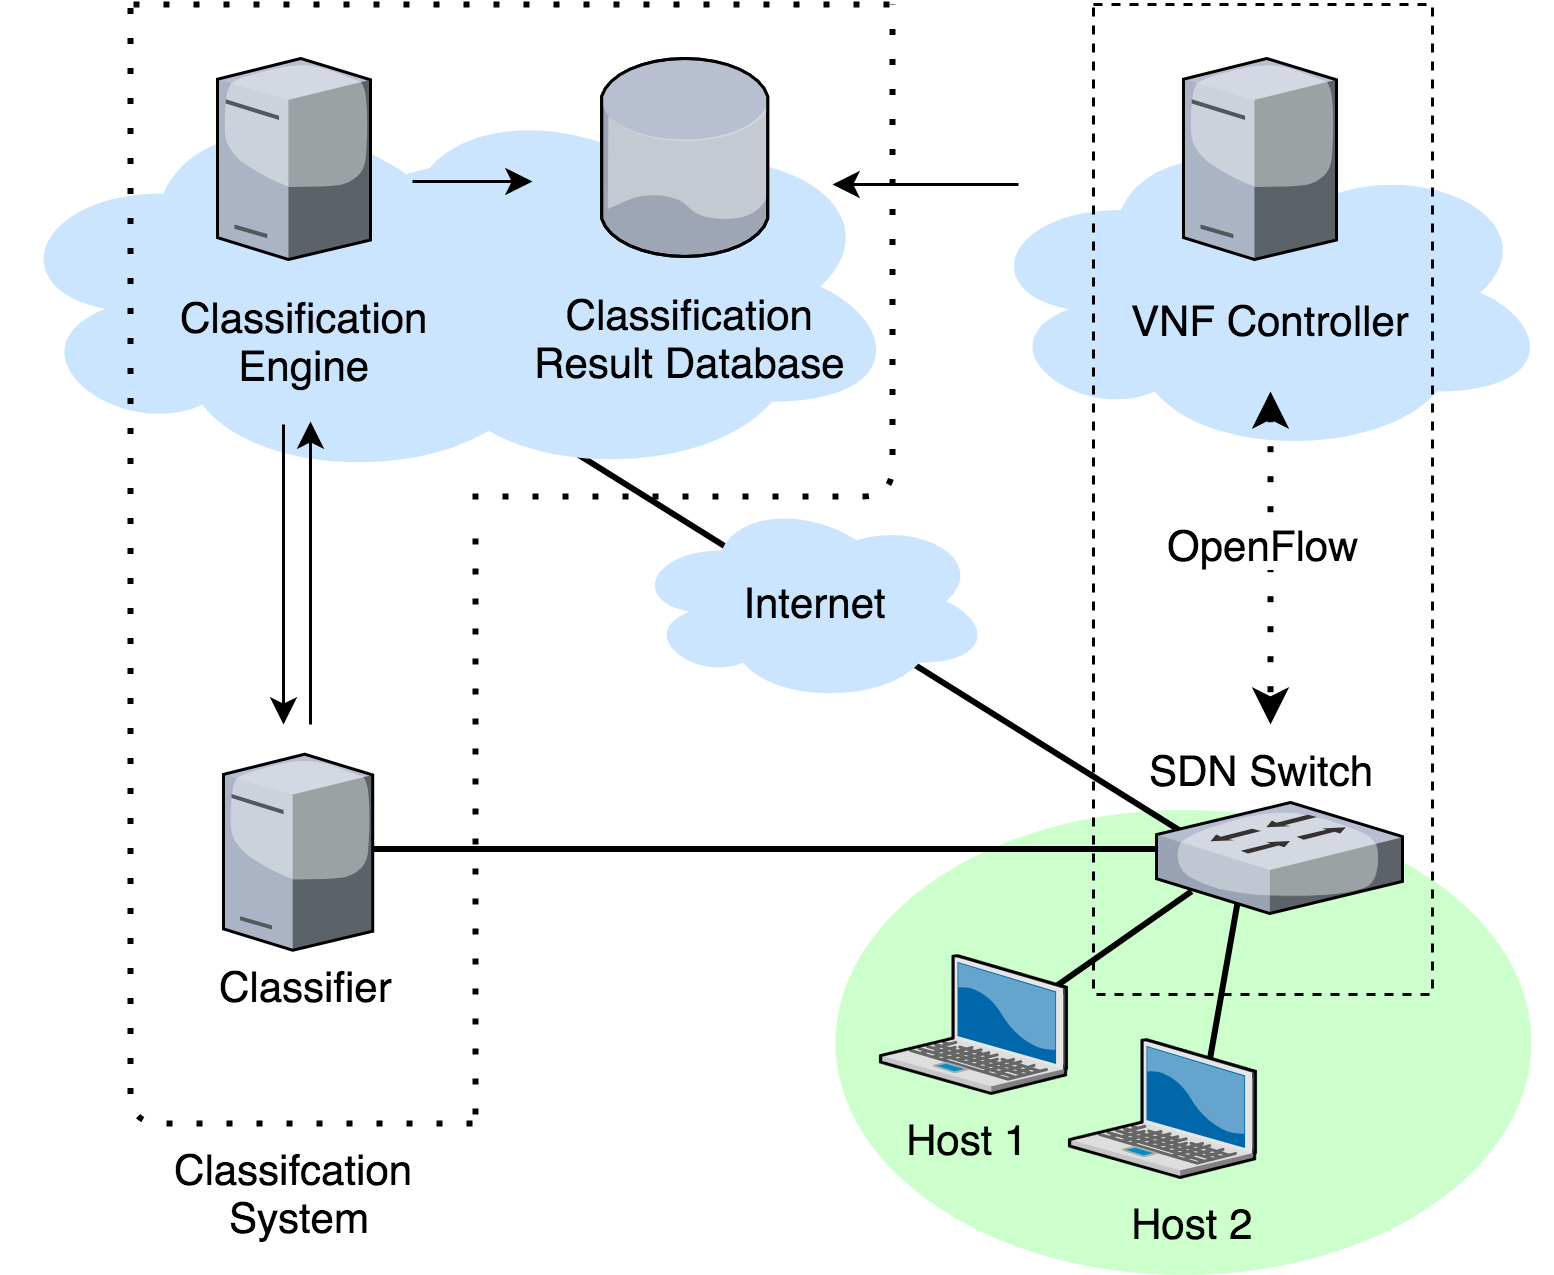
\includegraphics[width=0.4\textwidth]{./figures/classification_classifying}
\caption{Architecture of our application classification system in classification phase.}
\label{fig:class_classifying}
\end{figure}

\begin{figure}[!t]
\centering
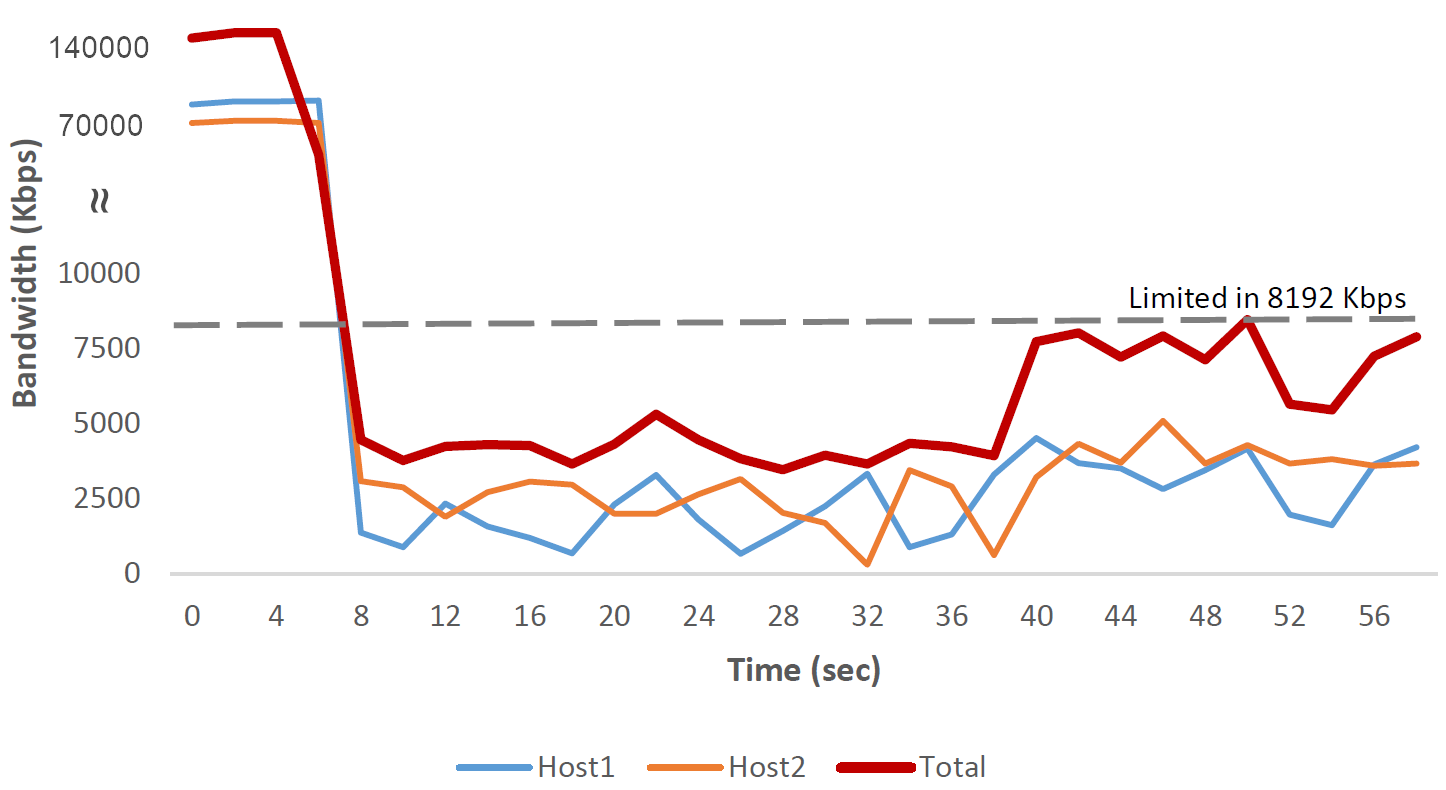
\includegraphics[width=0.4\textwidth]{./figures/mft_qos_rate_domain_app}
\caption{Limit the rate of FileZilla in a network domain.}
\label{fig:mft_qos_rate_domain_app}
\end{figure}



\subsection{Evaluation of QoS When Application Bandwidth Is Limited}
Our experimental environment is presented in Fig. \ref{fig:class_classifying}.
In our experimental environment, we mirror all traffic from the SDN switch to application classification system \cite{che-chuan-apnoms} and identify those flows belong to which application.
Then the application classification system uploaded the classification results to the database.
Subsequently, the controller received the results from the database and updated the flow information of the applications.
Therefore, we could use the flow information (5-tuple and classification results) to limit the application bandwidth.

We selected FileZilla to verify our function for limiting applications and there are two hosts (host 1 and host 2) in the same network domain.
Then we limited the bandwidth of FileZilla in this network domain. That is, the sum of bandwidths from host 1 and host 2.

As shown in Fig. \ref{fig:mft_qos_rate_domain_app}.
Initially, without limitation, the total bandwidth of FileZilla was approximately 140000 Kbps.
At the \nth{6} second, we limited the total bandwidth from FileZilla to 4096 Kbps.
Then we observed that the total traffic from FileZilla in this network domain immediately decreased.
Clearly, the total traffic from FileZilla was approximately 4096 Kbps.
At the \nth{38} second, we change the limitation from 4096 Kbps to 8192 Kbps and the total traffic from FileZilla increase to 8192 Kbps as expected.

Using this function for limiting applications, we can guarantee that the traffic in a network domain does not exceed the network capacity, thus preventing traffic congestion.




\section{Conclusion and Future Works}
The proposed vCPE framework enables deploying NFVs as edge of network and these VNFs are implemented with multiple flow table management model. In this way, the customers only need a SDN switch at local network, and some network functions that could not be realized by single table mechanism are also resolved. The results of the experiment show that the new VNF provides comparable performance compare with single table SDN application. The integration evaluation also demonstrates its flexibility to integrate with any other bonus application classification system, IDS or IPS.

However, the multiple flow table mechanism need more flow rules in the SDN switch and further research is needed. The mechanism uses more space in flow tables to gain more functionality. Also, the order of flow table of network functions must be fixed. As a future work, we plan to study further on the optimization for lower number of flow entries. We are still at an early stage of this approach and the full potential is yet to be revealed.


\section*{Acknowledgment}
This study is supported by the Ministry of Science and Technology (MOST) of Taiwan under grant numbers MOST 105-2221-E-007-083 and MOST 105-2622-8-009-008.


\bibliographystyle{ieeetr}
\bibliography{paper}


\end{document}
